\documentclass[14pt]{extarticle}
\usepackage[utf8]{inputenc}
\usepackage[T1]{fontenc}
\usepackage[spanish]{babel}
\usepackage{amsmath}
\usepackage{amsthm}
\usepackage{physics}
\usepackage{tikz}
\usepackage{float}
\usepackage[per-mode=symbol]{siunitx}
\usepackage{textcomp, gensymb}
\usepackage{multicol}
\usepackage{enumitem}
\usepackage[left=2.00cm, right=2.00cm, top=2.00cm, 
     bottom=2.00cm]{geometry}

\decimalpoint
\sisetup{bracket-numbers = false}
\DeclareSIUnit{\nothing}{\relax}

\title{\vspace*{-2cm}Prefijos para potencias de $10$\vspace{-5ex}}
\date{\today}
\begin{document}
\maketitle

\begin{table}[H]
\renewcommand{\arraystretch}{1.1}
\centering\
\begin{tabular}{c | c | c}
Potencia & Prefijo & Abreviatura \\ \hline
$\num{d-24}$ & yocto & $\unit{\yocto\nothing}$ \\ \hline
$\num{d-21}$ & zepto & $\unit{\zepto\nothing}$ \\ \hline
$\num{d-18}$ & atto & $\unit{\atto\nothing}$ \\ \hline
$\num{d-15}$ & femto & $\unit{\femto\nothing}$ \\ \hline
$\num{d-12}$ & pico & $\unit{\pico\nothing}$ \\ \hline
$\num{d-9}$ & nano & $\unit{\nano\nothing}$ \\ \hline
$\num{d-6}$ & micro & $\unit{\micro\nothing}$ \\ \hline
$\num{d-3}$ & mili & $\unit{\milli\nothing}$ \\ \hline
$\num{d-2}$ & centi & $\unit{\centi\nothing}$ \\ \hline
$\num{d-1}$ & deci & $\unit{\deci\nothing}$ \\ \hline
$\num{d3}$ & kilo & $\unit{\kilo\nothing}$ \\ \hline
$\num{d6}$ & mega & $\unit{\mega\nothing}$ \\ \hline
$\num{d9}$ & giga & $\unit{\giga\nothing}$ \\ \hline
$\num{d12}$ & tera & $\unit{\tera\nothing}$ \\ \hline
$\num{d15}$ & peta & $\unit{\peta\nothing}$ \\ \hline
$\num{d18}$ & exa & $\unit{\exa\nothing}$ \\ \hline
$\num{d21}$ & zetta & $\unit{\zetta\nothing}$ \\ \hline
$\num{d24}$ & yotta & $\unit{\yotta\nothing}$ \\ \hline
\end{tabular}
\end{table}
\begin{figure}[H]
    \centering
    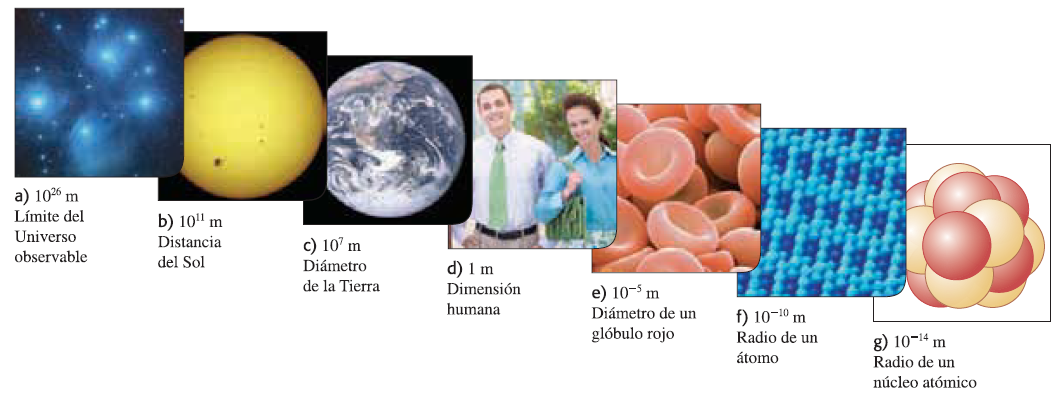
\includegraphics[scale=0.65]{Imagenes/Escala_Magnitud.png}
\end{figure}

\end{document}